\documentclass[11pt,titlepage]{article}
%\usepackage{eufrak,epsfig}
\usepackage{epsfig}
\usepackage{graphicx}
\usepackage{latexsym}
\usepackage{amssymb}
\usepackage{amsmath,amscd}
\usepackage{multirow} 
\usepackage{array}
\usepackage{caption}
\usepackage{subfig}
\usepackage{color}
\usepackage{url}
\usepackage{natbib}
\usepackage{rotating}
\usepackage{graphicx,lscape}
\usepackage{hyperref}
\usepackage{colortbl}
\usepackage{tikz}
\usetikzlibrary{matrix}
\usepackage{indentfirst}
\usepackage{colortbl}
\usepackage{bm}
\usepackage{kotex}
\usepackage[margin=3.1cm]{geometry}
\long\def\comment#1{} 

%\nofiles
\newcommand{\rb}[1]{\raisebox{-.5em}[0pt]{#1}}
\renewcommand{\baselinestretch}{1.7}
\renewcommand{\mid}{\, | \ , }
\newcommand{\eighth}{{\textstyle \frac{1}{8}}}

\newcommand{\by}{\mbox{\boldmath $y$}}
\newcommand{\bx}{\mbox{\boldmath $x$}}
\newcommand{\bd}{\mbox{\boldmath $d$}}
\newcommand{\bv}{\mbox{\boldmath $v$}}
\newcommand{\bu}{\mbox{\boldmath $u$}}
\newcommand{\bl}{\mbox{\boldmath $\ell$}}
\newcommand{\bW}{\mbox{\boldmath $W$}}
\newcommand{\bX}{\mbox{\boldmath $X$}}
\newcommand{\bY}{\mbox{\boldmath $Y$}}
\newcommand{\bA}{\mbox{\boldmath $A$}}
\newcommand{\bV}{\mbox{\boldmath $V$}}
\newcommand{\bL}{\mbox{\boldmath $L$}}
\newcommand{\bdm}{\begin{displaymath}}
\newcommand{\edm}{\end{displaymath}}
\newcommand{\bbeta}{\mbox{\boldmath $\beta$}}
\newcommand{\btheta}{\mbox{\boldmath $\theta$}}
\newcommand{\btt}{\mbox{\boldmath $\theta$}}
\newcommand{\bep}{\mbox{\boldmath $\epsilon$}}

\newcommand{\balpha}{\mbox{\boldmath $\alpha$}}
\newcommand{\bxi}{\mbox{\boldmath $\xi$}}
\newcommand{\bXi}{\mbox{\boldmath $\Xi$}}
\newcommand{\bmu}{\mbox{\boldmath $\mu$}}
\newcommand{\bgamma}{\mbox{\boldmath $\gamma$}}

\newcommand{\bphi}{\mbox{\boldmath $\phi$}}
\newcommand{\bpsi}{\mbox{\boldmath $\psi$}}
\newcommand{\C}{{\rm Cov}}

\newcommand{\bld}[1]{\mbox{\boldmath $#1$}}
\newcommand{\bmmu}{\bld \mu}
\newcommand{\bbf}{\bld f}
\newcommand{\bbe}{\bld e}
\newcommand{\bbg}{\bld g}
\newcommand{\bbx}{\bld x}
\newcommand{\bbz}{\bld z}
\newcommand{\cC}{{\cal C}}
\newcommand{\cB}{{\cal B}}
\newcommand{\cH}{{\cal H}}

\renewcommand{\baselinestretch}{1.8}
\setlength\arraycolsep{2pt}
\linespread{1.5}

\title{\bf Lifting Scheme for Data in River Networks
\medskip
}

\author{
Seoncheol Park \\
Pacific Climate Impacts Consortium\\
University of Victoria\\
Victoria, BC V8W 2Y2, Canada\\
\\
Hee-Seok Oh \\
Department of Statistics\\
Seoul National University\\
Seoul 08826, Korea\\
\\
}
\date{Draft: version of \today}

\begin{document}

\maketitle


\begin{abstract}
This paper presents a new multiscale method for analyzing water pollutant data located in river networks. The main idea of the proposed method is to adapt the conventional lifting scheme, one of the second-generation wavelets, reflecting the characteristics of streamflow data in the river network domain. Due to the complexity of the data domain structure, it is difficult to apply the lifting scheme to the streamflow data directly. To solve this problem, we propose a new lifting scheme algorithm for streamflow data that incorporates flow-adaptive neighborhood selection, flow proportional weight generation, and flow-length adaptive removal point selection. A non-decimated version of the proposed lifting scheme is also provided. The simulation study demonstrates that the proposed method successfully performs a multiscale analysis of streamflow data. Furthermore, we provide a real data analysis of water pollutant data observed on the Geum-River basin compared to the existing smoothing method. 

\vskip 7mm

\noindent {\it Keywords}: Lifting scheme; River network; Smoothing; Spatial adaptation; Spatial modeling; Streamflow data. 

\end{abstract}

\section{Introduction}\label{sec:intro}

Environmental monitoring is a collection of observations and studies for the evaluation of environmental data \citep{Artiola2004}. Humans now know that the environment is crucial to our health and survival. Therefore, we cannot overemphasize  environmental monitoring for humans. One of the main areas of environmental monitoring is water quality management. As human activities increase, more environmental costs are needed to rehabilitate water. Therefore, it is important to analyze the characteristics of water pollutants. 

This paper focuses on the environmental pollutant called Total Organic Carbon (TOC, mg/L). Recently, the Korean Ministry of Environment announced that they changed the water pollution index for monitoring wastewater treatment performance of facilities from chemical oxygen demand (COD) to TOC. According to the ministry, it cannot measure all organic matters in the water. However, using TOC can compensate for these shortcomings. Therefore, analyzing TOC data is meaningful to society.  The National Institute of Environmental Research (NIER) under the Ministry of Environment operates a water environment information system to monitor water quality. This system provides ``Environment standard", which is a good guideline for the amount of TOC listed in Table \ref{table:table1}.

\begin{table}[!h]
	\centering	
	\caption{Environment standard for TOC provided by Water Environment Information System (WEIS).}
	\begin{tabular}{|l|c|c|c|c|c|c|c|}
		\hline
		Status & Very good & Good & Slightly better & Normal & Poor & Bad & Very bad \\ \hline
		%WEIS level & %\cellcolor{blue}\textcolor{white}{Ia} & %\cellcolor{cyan}\textcolor{white}{Ib} & %\cellcolor{green}\textcolor{white}{II} & %\cellcolor{gray}\textcolor{white}{III} & %\cellcolor{yellow}IV & \cellcolor{orange}V %& \cellcolor{red}VI \\ \hline
		TOC (mg/L) & $\leq 2$ & $\leq 3$ & $\leq 4$ & $\leq 5$ & $\leq 6$ & $\leq 8$ & $>8$ \\ \hline
\end{tabular}
	\label{table:table1}
\end{table}

\begin{figure}
	\centering
	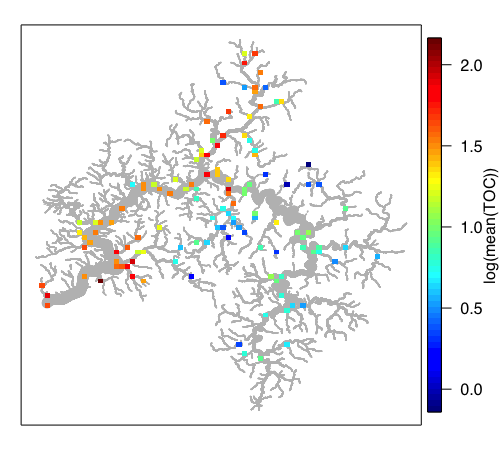
\includegraphics[width=0.6\textwidth]{Stream_result/Figure01.png}
	\vspace{-2mm}
	\caption{TOC data on the Geum-River network. Gray lines mean streamflow segments with different weights represented by their widths, and colored points mean logarithm values of TOC means from December 2011 to November 2017 in 127 observation sites.}
	\label{fig:fig1}
\end{figure}

From Figure \ref{fig:fig1}, we can find some characteristics of the water quality index: (i) The TOC index is located in the river network. It means that observations are correlated across the river network, not the usual $\mathbb{R}^2$ domain. Most statistical models are interested in analyzing a spatial region, a subset of $\mathbb{R}^2$, where Euclidean distance works well. On the other hand, for the streamflow data in Figure \ref{fig:fig1}, Euclidean distance does not work well as a natural metric. (ii) As shown in Figure \ref{fig:fig1}, the data have spatially inhomogeneous features in various dependent structures along with the river network. (iii) The data are irregularly observed in the river network.  

Therefore, any such method of representing the above data should have the following features: (i) It is capable of effectively represent streamflow data in the river network. (ii) It provides a spatially adaptive framework to estimate the inhomogeneous underlying function by reflecting the inherent multiscale characteristics of data. (iii) It applies to scattered data in the river network. In this paper, we would like to propose a multiscale method that satisfies all of the features mentioned above. 

In this paper, we assume that observations are a set of scattered data $(x_i, y_i)$, $i=1,\ldots,n$, as shown in Figure \ref{fig:fig1}, from model 
\begin{equation}\label{eq:scattered}
y_i = g(x_i)+\varepsilon_i, 
\end{equation}
where $x_i$ denotes the locations of observations in the data domain, $\varepsilon_i$ are the measurement errors, and $g$  denotes an unknown underlying function of interest. Our goal is to estimate the underlying field $g(x)$ for every location $x$ on the river network. In other words, for the case in Figure \ref{fig:fig1}, we would like to represent the underlying field of the water quality index in the river network domain. 

In the literature, there exist some studies of streamflow data analysis. \cite{VerHoef(2006)} proposed the use of stream distance  defined by the shortest distance between two locations on river networks, as a reasonable distance measure for data analysis on the river network. They showed that it could construct a large class of valid spatial autocovariance models using the stream distance. They also suggested a kernel convolution-based method generates a class of covariance models for streamflow data. \cite{ODonnell2014} used nonparametric flexible regression approaches, such as kernel methods and penalized splines, to build spatio-temporal models in river networks. They suggested a piecewise simple regression analysis by dividing the network into a large number of small pieces called ``stream segments".  They provided regression-based stream data estimates  assuming that the function values $g$'s are constant within the same stream segments.

Meanwhile, due to the complexity of the river network data, it is not easy to fully understand the underlying structure of the  data. The multiscale analysis is a possible way to solve such a problem by considering the multiresolution of data. As conventional multiscale methods, wavelets are the most popular choice. However, wavelets do not properly work when the data are not observed on regular grids, or the number of observations is not dyadic, i.e., $n=2^{J}$, for some $J\in \mathbb{Z}$. To overcome these problems, \citet{Sweldens1996} and \citet{Sweldens1998} proposed a kind of the second-generation wavelet called ``lifting scheme''. The lifting scheme has been extensively studied in signal processing and image analysis \citep{Jansen2005}. 

However, there is a limit that all of the previous works cannot provide a multiscale structure for river network data. As far as we know, there is no direct literature describing multiscale methods for river network data. In this paper, a new lifting method for river network data is proposed by combining the conventional lifting method and novel modifications of neighborhood selection, filter prediction, and removal point selection, taking into account the characteristics of the data. The proposed method has two advantages. First, by following the argument of the lifting scheme, it gives a multiscale structure of river network data. Second, the proposed method is advantageous compared to the conventional smoothing methods for river networks from the signal denoising point of view.

The rest of the paper is organized as follows. Section \ref{sec:lifting} reviews the existing lifting schemes and smoothing method in the river network. Section \ref{sec:data} describes the river network data used in this study. Section \ref{sec:streamflowliftingscheme} presents a new method termed ``streamflow lifting scheme''. Simulation studies and real data analysis are conducted in Sections \ref{sec:streamflowsimulationdata} and \ref{sec:streamflowrealdata} to evaluate the proposed method. Finally, concluding remarks are provided in Section \ref{sec:streamflowsummary}.

\section{Backgrounds}\label{sec:lifting}

\subsection{Lifting scheme}

In this section, we briefly summarize the concept of lifting scheme for self-contained material. Suppose that we observe a set of $n$ irregular locations $\bm{x}=(x_{1},\ldots, x_{n})^{T}$, where the length of the data $(=n)$ may not be dyadic. Assume that we have function values $y_1,\ldots, y_n$ at every location. We want to construct a multiresolution transform at the $j-1$th level, given the $j$th level data $\bm{y}_{j}$. The lifting scheme consists of the following four steps:
\begin{enumerate}
\item \textbf{Split}: At the level $j-1$, divide $\bm{y}_{j}$ into two subsets, $\mathcal{P}_{j-1}$ and $\mathcal{U}_{j-1}$. 

\item \textbf{Predict}: Predict every sample $y_{j,i}\in\mathcal{P}_{j-1}$ from $y_{j,k}\in\mathcal{U}_{j-1}$ with a prediction filter $\mathbf{p}_{j-1,i}$, and store the prediction error $d_{j-1,i} = y_{j,i} - \hat{y}_{j,i} = y_{j,i} - \sum_{k \in \mathcal{N}_{j-1,i}\cap \mathcal{U}_{j-1}}p_{j-1,i,k}y_{j,k},$ where $\mathcal{N}_{j-1,i}$ is the set of neighbors of node $i$, $\hat{y}_{j,i}$ represents the predicted value constructed from $\mathcal{U}_{j-1}$ neighbors of node $i$. Note that $i$ and $k$ denote location in $\mathcal{P}_{j-1}$ and $\mathcal{U}_{j-1}$, respectively. 

\item \textbf{Update}: Update  the $j-1$th level data $y_{j-1,k}$ in $\mathcal{U}_{j-1}$ with an appropriate update filter $\mathbf{u}_{j-1,k}$, that is, 
	$y_{j-1,k} = y_{j,k}+\sum_{i\in\mathcal{N}_{j-1,k}\cap \mathcal{P}_{j-1}}u_{j-1,k,i}d_{j-1,i}.$ 
	
\item \textbf{Repeat}: Repeat the above steps until the desired resolution level is achieved.
\end{enumerate}

By performing these steps, we construct coarse signals of data from updated subsamples. Meanwhile, the reverse version of the lifting scheme can be easily obtained by undoing the forward scheme operations at the level $j-1$: (i) Undo update: $ y_{j,k} = y_{j-1,k} - \sum_{i\in\mathcal{N}_{j-1,k}\cap \mathcal{P}_{j-1}}u_{j-1,k,i}d_{j-1,i}.$ (ii) Undo predict: $d_{j,i} = d_{j-1,i} + \sum_{k\in\mathcal{N}_{j-1,i}\cap \mathcal{U}_{j-1}}p_{j-1,i,k}y_{j,k}.$ (iii) Undo split. (iv) Repeat the above steps at the next level.

There are several crucial components in the construction of the lifting scheme.
\begin{itemize}
	\item \textbf{The number of removing points at ones} $(|\mathcal{P}|)$: The user should select how many points remain at the next (coarser) level.  
	
	\item \textbf{Prediction filter}: It is essential to choose a prediction filter in the procedure. Haar (local constant), local linear, local polynomial, or inverse distance weight are frequently used in the literature.  
	
	\item \textbf{Removal order of points}: When removing the points, it is crucial to determine the order in which points are removed. It relates to the question of whether or not what is essential to represent the underlying field. 	
	
	\item \textbf{Neighborhood selection}: It is important to select multiple neighbors to construct a prediction filter. Too many neighbors make it difficult to understand the local behavior of the data, while too few neighbors yield a bias to predict each node.
\end{itemize}

\subsubsection{Lifting one coefficient at a time (LOCAAT)}\label{sec:LOCAAT}
We now review the lifting one coefficient at a time (LOCAAT) algorithm of \cite{Jansen2009}. The LOCAAT algorithm constructs a removal order of data points and sequentially decomposes the data with the order. Suppose we have the values $y_{1}, \ldots, y_{n}$, sampled at $n$ irregularly spaced points $x_{1}, \ldots, x_{n}$ on the real line. Lifting scheme approximates the function $g$ in (\ref{eq:scattered}) as 
\[
\tilde{g}(y) = \sum_{k=1}^{n} c_{n,k} \phi_{n,k}(x),
\] 
where $c_{n,i}:=g(x_{i})$, $\phi_{n,k} (x_{i}) = \delta_{i,k}$ for $k,i \in \{1, \ldots, n\}$, and $\delta_{i,k}$ denotes the Kronecker delta. 

The LOCAAT algorithm first defines the index set of the scaling coefficients as $\mathcal{U}_{n} = \{1,\ldots,n\}$ and the index set of wavelet coefficients as $\mathcal{P}_{n} = \emptyset$. At the next step $n-1$, a point to be lifted is selected and denoted as $j_{n}$, which is the point to be removed from the current set of scaling coefficients and to be converted into a detailed coefficient. The new set of indices corresponding to the scaling coefficients is $\mathcal{U}_{n-1} = \mathcal{U}_{n} \backslash \{j_{n}\}$, while $\mathcal{P}_{n-1} = \{ j_{n}\}$ is the index set of the wavelet coefficient constructed at this stage.

To select the point to be lifted, \cite{Jansen2009} used the minimum of the integral of scaling function $\phi_{n,k}$, $I_{nk}$, as an appropriate measure. In this study, length or volume is considered as an appropriate measure. Figure \ref{fig:removeI} shows a toy example that selects a point to be lifted by the LOCAAT algorithm. A, B, C, and D denote locations. The area of each point can be defined by dividing the real line into four blocks using the midpoint marked by the vertical line. The LOCAAT algorithm selects among the candidates a point with the smallest area corresponding to the length of each block in the one-dimensional data area. In this example, a point of $B$ is selected to be removed. 
\begin{figure}
	\vspace{-5mm}
	%\centering
	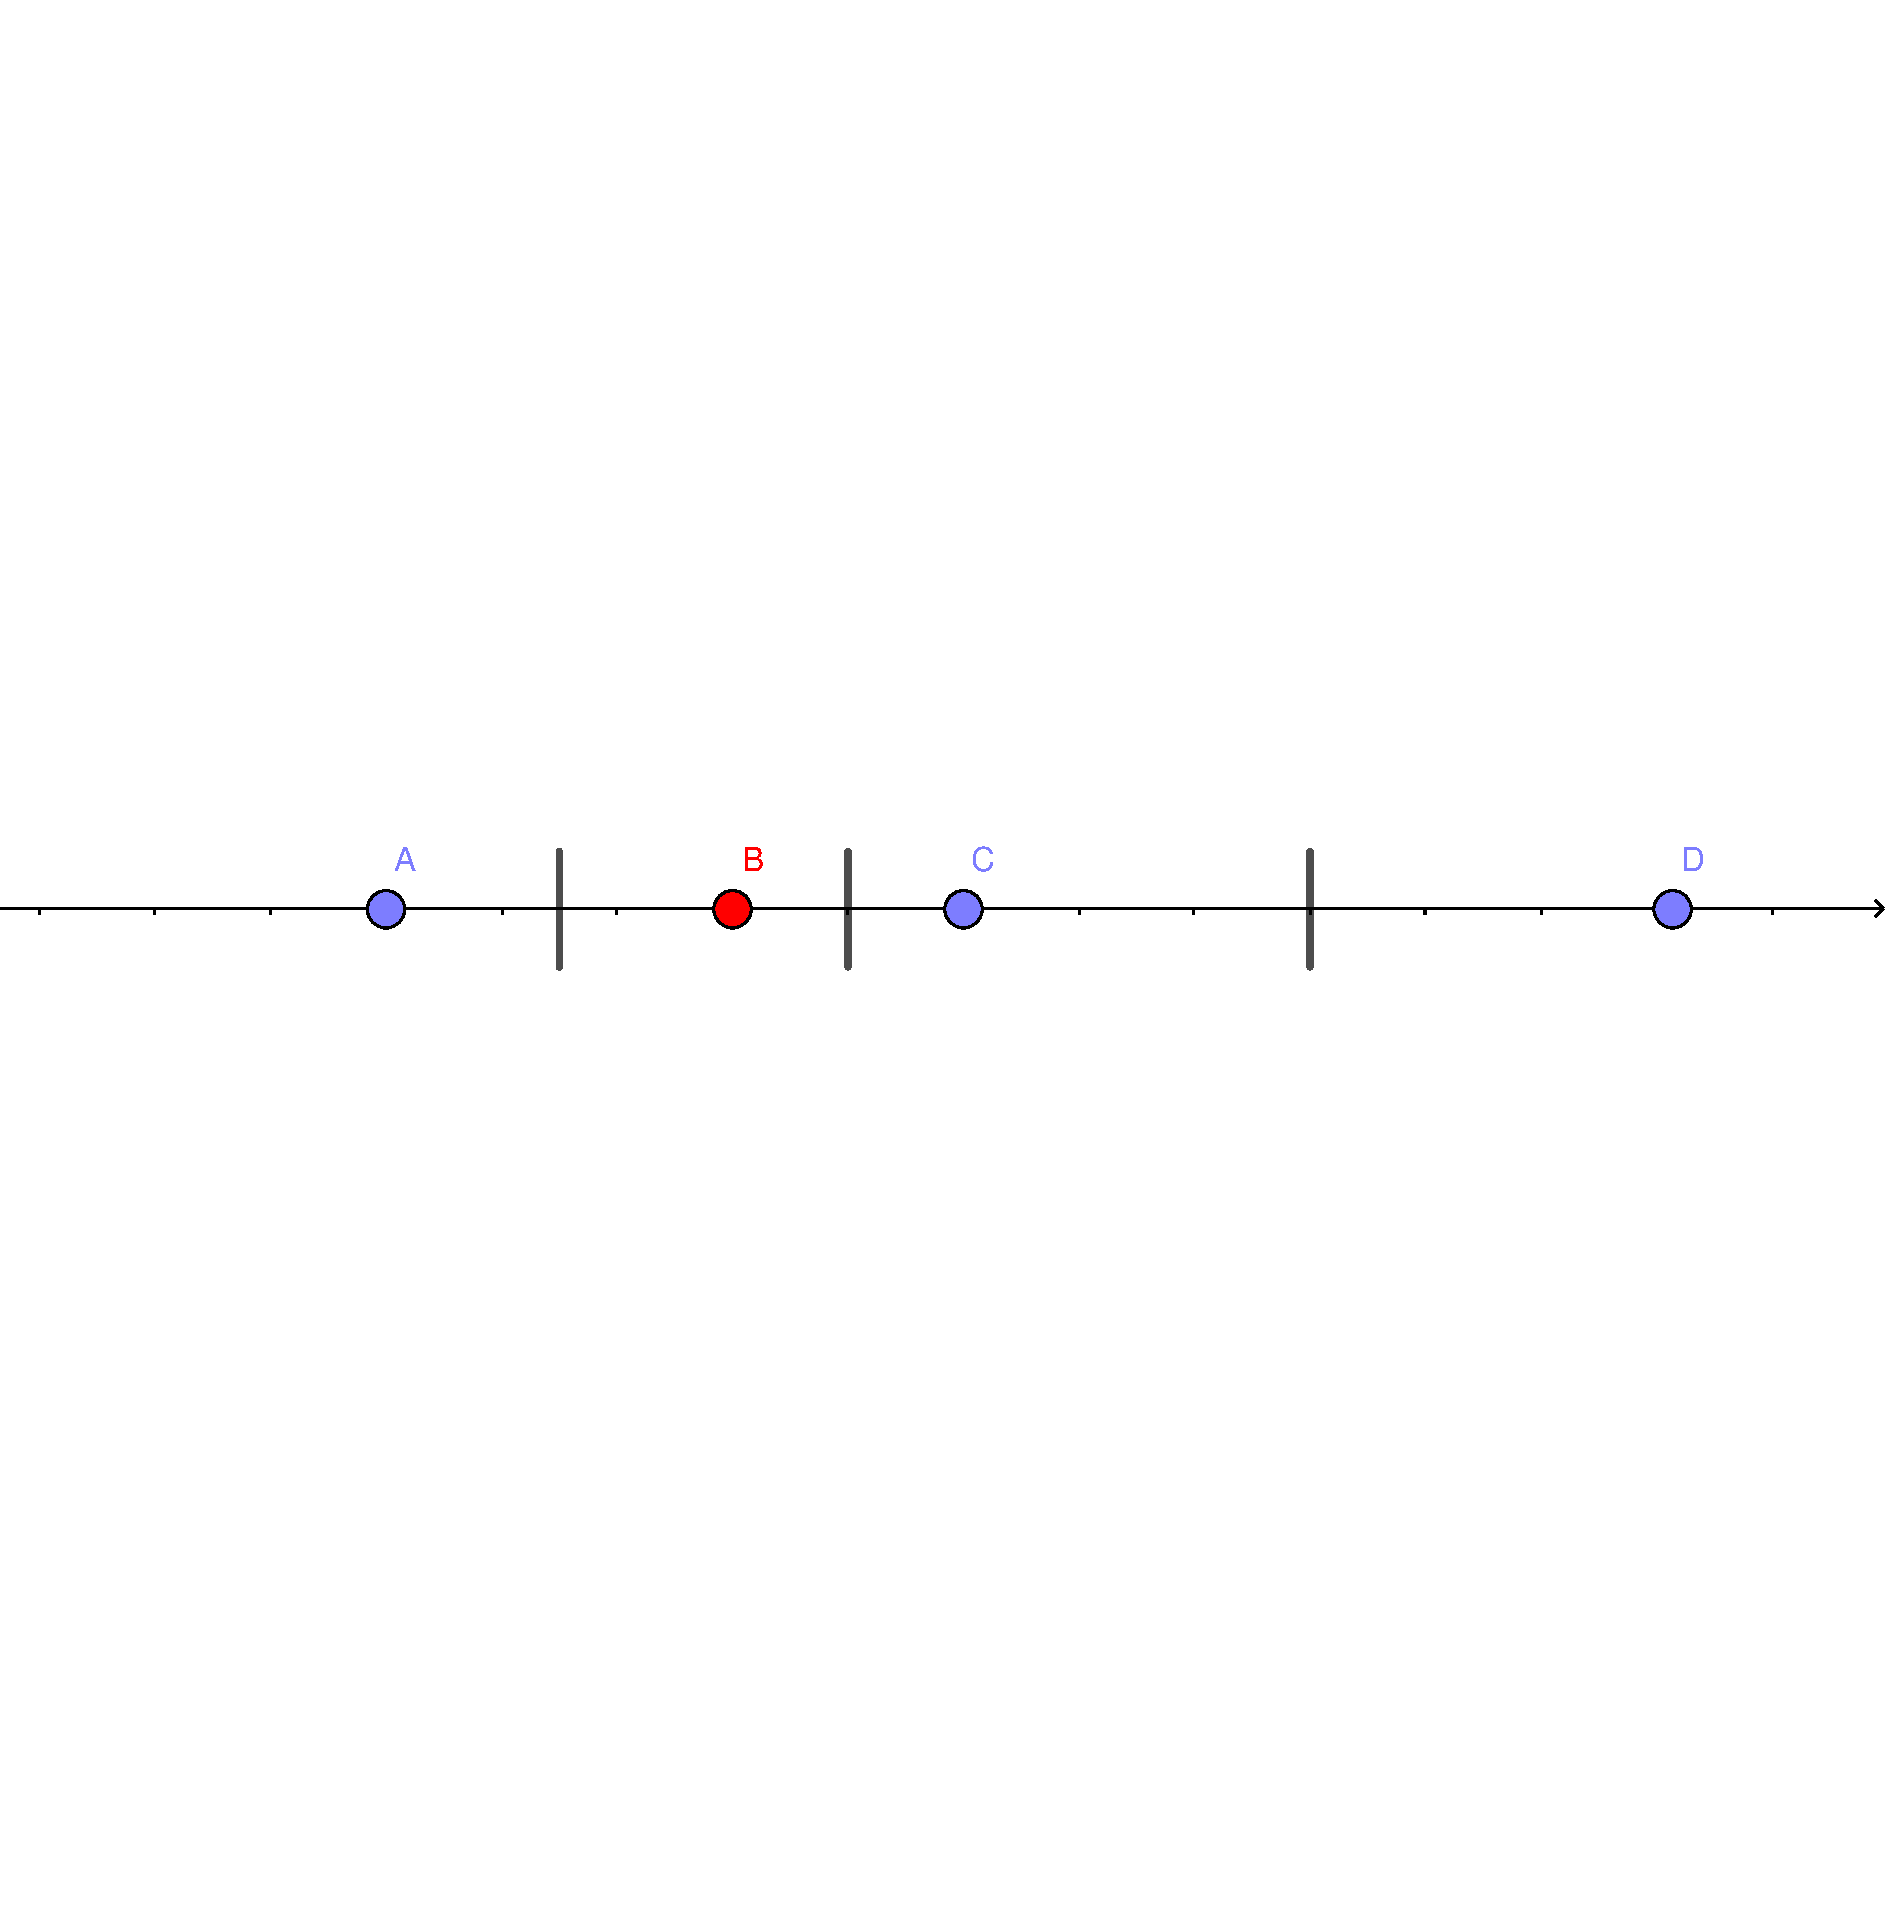
\includegraphics[width=0.95\textwidth]{Stream_result/horzline.pdf}
	\caption{Illustration of the removal point selection of lifting scheme in the real line.}
	\vspace{-3mm}
	\label{fig:removeI}
\end{figure}
For the configuration of update filters, \citet{Jansen2009} proposed a minimum norm solution-based update weights at level $r$ due to the numerical stability, 
\begin{equation}
\label{eqn:updatefilter}
b_{j}^r = I_{r i_r}I_{r-1,j}/ \sum_{k\in \mathcal{N}_r} I_{r-1,k}^2,
\end{equation}
where $i_r$ is an index of the candidate points for removal. 

\subsubsection{Other lifting schemes}\label{subsec:otherlifting}
\cite{Nunes2006} proposed a new lifting scheme called ``adaptive lifting''. The key ingredients of the adaptive lifting are the data-adaptive selection of the removal order and the neighborhood size in the lifting prediction step. Especially, they considered linear, quadratic, and cubic regression-based prediction filter in each step in LOCAAT and selected a filter which generates the smallest absolute value of detail coefficient. In the same way, we can decide the optimal neighborhood size of each predict step. Through these modifications, \cite{Nunes2006} flexibly constructed prediction filters in the one-dimensional signal denoising setting.

In the lifting scheme, it is not easy to find the optimal removal sequence because there is no optimal removal order in terms of minimizing the mean square error. To enhance the performance of the lifting scheme in nonparametric regression settings, \cite{Knight2009} proposed a ``nondecimated'' concept in lifting transform. It borrows the idea from a nondecimated wavelet transform that uses over-determined basis functions to improves the performance of the wavelet transform. \cite{Knight2009} generated several removal order sequences called paths. They generated $Q$ different removal orders by permutation. Following notations of \cite{Knight2009}, let $\hat{g}^{(q)}(x)$ be the estimate of the unknown function $g$ at locations $x$, using the $q$th path. They showed that an averaged estimator $$\hat{\bar{g}}(x_{i}) = \frac{1}{Q}\sum_{q=1}^{Q}\hat{g}^{(q)}(x_{i}), \qquad{\forall i = 1,\ldots , n}
$$
could reduce the error between the true signal and its estimator. For a better smoothing, \cite{Knight2009} further selected a few paths that provide lower approximated average square errors $\widehat{\text{ASE}}$,
\[
\widehat{\text{ASE}}(\hat{g}^{(q)},g) =\frac{1}{n}\sum_{i=1}^{n}\{ \hat{g}^{(q)}(x_i) -\hat{\bar{g}}(x_i) \}^{2}.
\]

\subsection{Shrinkage in the lifting scheme}

Lifting schemes have also been applied to nonparametric regression problems by incorporating a shrinkage approach. The main idea of shrinkage is based on the assumption that the true signal information is contained only in large values of the $\mathbf{d}$ elements. Thus, by setting the $d$ coefficient less than a specific threshold to zero, the reconstruction results may be more similar to the true signal.
\comment{
\begin{figure}
	\centering
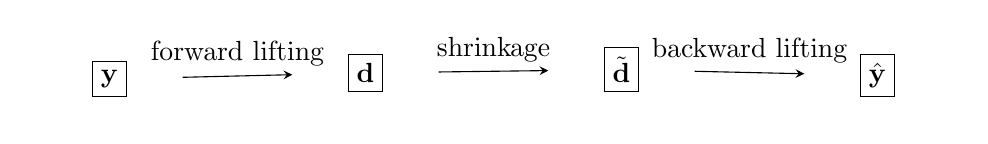
\begin{tikzpicture}
\matrix (m) [matrix of math nodes,row sep=3em,column sep=4em,minimum width=5.25em]
{
	%F_t(x) & F(x) \\
	%A_t & A 
	\framebox[2\width]{$\mathbf{y}$} & \framebox[2\width]{$\mathbf{d}$} & \framebox[2\width]{$\tilde{\mathbf{d}}$} & \framebox[2\width]{$\hat{\mathbf{y}}$}\\};
\path[-stealth]
(m-1-1) edge node [above] {forward lifting} (m-1-2)
(m-1-2) edge node [above] {shrinkage} (m-1-3)
%(m-1-2) edge node [below] {(ex. EbayesThresh)} (m-1-3)
(m-1-3) edge node [above] {backward lifting} (m-1-4);
%(m-2-1.east|-m-2-2) edge node [below] {$\mathcal{B}_T$}
%node [above] {$\exists$} (m-2-2)
%(m-1-2) edge node [right] {$\mathcal{B}_T$} (m-2-2);
%edge [dashed,-] (m-2-1);
\end{tikzpicture}
\caption{Illustration of lifting scheme with shrinkage.} \label{fig:tikzpicture01}
\end{figure}
}

In the proposed streamflow lifting scheme to be discussed in Section 4, we use the same shrinkage strategies used in \cite{Nunes2006} and \cite{Knight2009}. There are several types of shrinkage approaches. In this paper, we focus on the median and hard thresholds, which are implemented as \texttt{median} and \texttt{hard} in \texttt{adlift} and \texttt{nlt} package in R. To use the lifting scheme, one must decide the number of scaling coefficients to be kept in the final representation of the initial signal. The user also specifies \texttt{nkeep} in \texttt{adlift} and \texttt{nlt} package in R. In this paper, we use the fully decomposed result (\texttt{nkeep=2}) in \cite{Knight2009}, which produces $(n-2)$ detail coefficients in the length-$n$ dataset. 
 

\subsection{Smoothing method on river networks}
In this subsection, we briefly summarize the work of \cite{ODonnell2014}. One of the key ideas of \cite{ODonnell2014} is to simplify the information in a given network using the concept of stream segments. They also suggested a penalize spline-based method with spatial, seasonal, temporal, and interaction bases. This paper focuses on the analysis of the spatial behavior of pollutants, taking into account the structure of river networks. For this purpose, we consider a straightforward spatial additive model as 
\begin{equation}\label{eqn:spatialsimpleadditive}
y_{i} = \mu + m_{x}(x_i) + \varepsilon_{i} = g(x_i) + \varepsilon_{i},
\end{equation}
where $m_x$ describes spatial trends. The main idea of the spline method is to use a set of basis functions to estimate $g$ in  (\ref{eq:scattered}). So, with $p$ basis functions, the estimator is $\hat{g}(x) = \sum_{j=1}^{p}\beta_{j} \phi_{j}(x)$. \cite{ODonnell2014} used a P-spline basis, which is a penalized version of a B-spline basis. More specifically, a B-spline model is formulated as $\mathbf{y}=B\boldsymbol{\beta} +\boldsymbol{\varepsilon}$, where $B= (1, B_s)$, where $B_{s}$ is a design matrix of spatial components, and $\boldsymbol{\beta}$ is an $n\times p$ response vector. The model is fitted by minimizing the following penalized sum of squares
\begin{equation}\label{eqn:ODonnellsmoothing}
(\mathbf{y}-B\boldsymbol{\beta})^{T}(\mathbf{y}-B\boldsymbol{\beta}) + \lambda\boldsymbol{\beta}^{T}D^{T}D\boldsymbol{\beta},
\end{equation} 
where $D$ denotes the penalty matrix. The solution of (\ref{eqn:ODonnellsmoothing}) is $\hat{\boldsymbol{\beta}} = (B^{T}B+ \lambda D^{T} D)^{-1}B^{T}\mathbf{y}$, where $\lambda$ is a smoothing parameter. For the optimal value of $\lambda$, \cite{ODonnell2014} selected $\lambda$ to minimize $\log(\hat{\sigma}^{2}) + 1 + \frac{2+2\text{df}}{n-\text{dof}-2}$, where $\text{df}$ denotes the degree of freedom. For the detailed information of smoothing methods in the stream network. refer to \cite{ODonnell2014}. 


\section{Geum-River TOC data}\label{sec:data}

%catchment: 유역 (watershed 라고도 )
The data used in this paper are observed in the Geum-River basin located in the heart of South Korea. See Figure \ref{fig:studyarea}(a). According to the Water Environment Information System operated by the Ministry of Environment, the Geum-River basin is divided by 14 sub-regions, called catchments, which are plotted with solid lines in Figure 3(a) and (b). All 14 catchments are also divided into several sub-catchments, which are plotted with dotted lines in Figure \ref{fig:studyarea}(a) and (b). Among them, the Miho-Cheon catchment marked by orange in Figure \ref{fig:studyarea}(b) is one of the sub-regions. It contains many observational stations compared to other catchments, and there are several cities and factories around it. We believe it is meaningful to take a closer look at the area. This river network is also applied to build a network model for simulation studies in Section 5. 

The orange lines in the Miho-Cheon catchment of Figure \ref{fig:studyarea}(b) represent stream segments defined by lines between junctions of the river network \citep{VerHoef(2006), VerHoef(2010)}. We note that there are 113 streaㅡm segments and 28 observation stations in the Miho-Cheon catchment. The Geum-River network has a total of 942 stream segments and 127 observation points. 

\begin{figure}[!th]
	\centering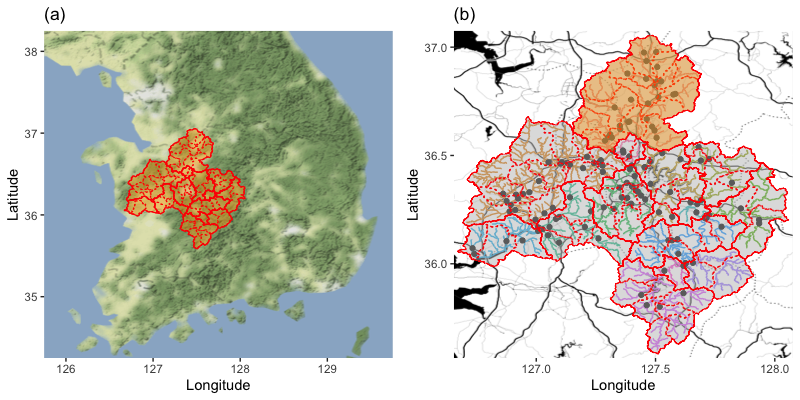
\includegraphics[width=\textwidth]{Stream_result/Studyarea_small.png}
	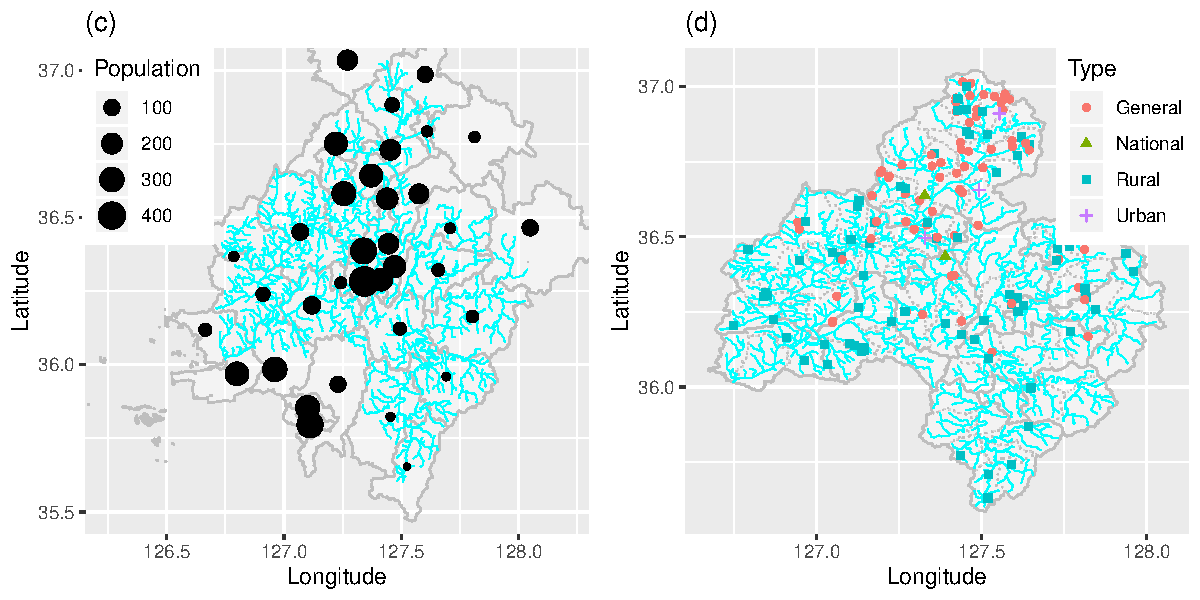
\includegraphics[width=\textwidth]{Stream_result/Studyarea_additional.pdf}\caption{(a) The Geum-River catchments in South Korea marked by red lines. (b) The Enlarged figure of (a). Black dots are 127 observation points. (c) Populations (2017/12/31, thousands) in the Geum-River basin. (d) Locations of industrial areas in the Geum-River basin.}
	\label{fig:studyarea}
\end{figure}

Figure \ref{fig:studyarea}(c) shows the cities, counties, and districts populations located in the Geum-River basin. Note that these administrative areas do not fully match the Geum-River catchments. From Figure \ref{fig:studyarea}(c), we observe that most of the populations are concentrated in the Northern and Central parts of the Geum-River basin. Figure \ref{fig:studyarea}(d) shows the locations of industrial areas in Geum-River basins. Note that general, national, and urban industrial sites are clustered in the Miho-Cheon and its nearby areas. Therefore, it is possible to assume that many water pollutants will occur in the Miho-Cheon and its adjacent river basin.


\section{Streamflow lifting scheme}\label{sec:streamflowliftingscheme}

This section presents our procedure to construct a new lifting scheme for streamflow data by modifying the LOCAAT algorithm of  \citet{Jansen2009} to adapt some characteristics of streamflow data. Our main idea is to develop a multiscale method for streamflow data analysis by incorporating the idea of \cite{Nunes2006} into \cite{ODonnell2014}. The necessary modifications for developing the streamflow lifting scheme are as follows: (i) performing a network-adaptive neighborhood selection, (ii) constructing a prediction filter with flow-adaptive weighted averages, and (iii) determining a removal order by defining a proper contribution measure of each observation point to the river network.

\begin{figure}
	\centering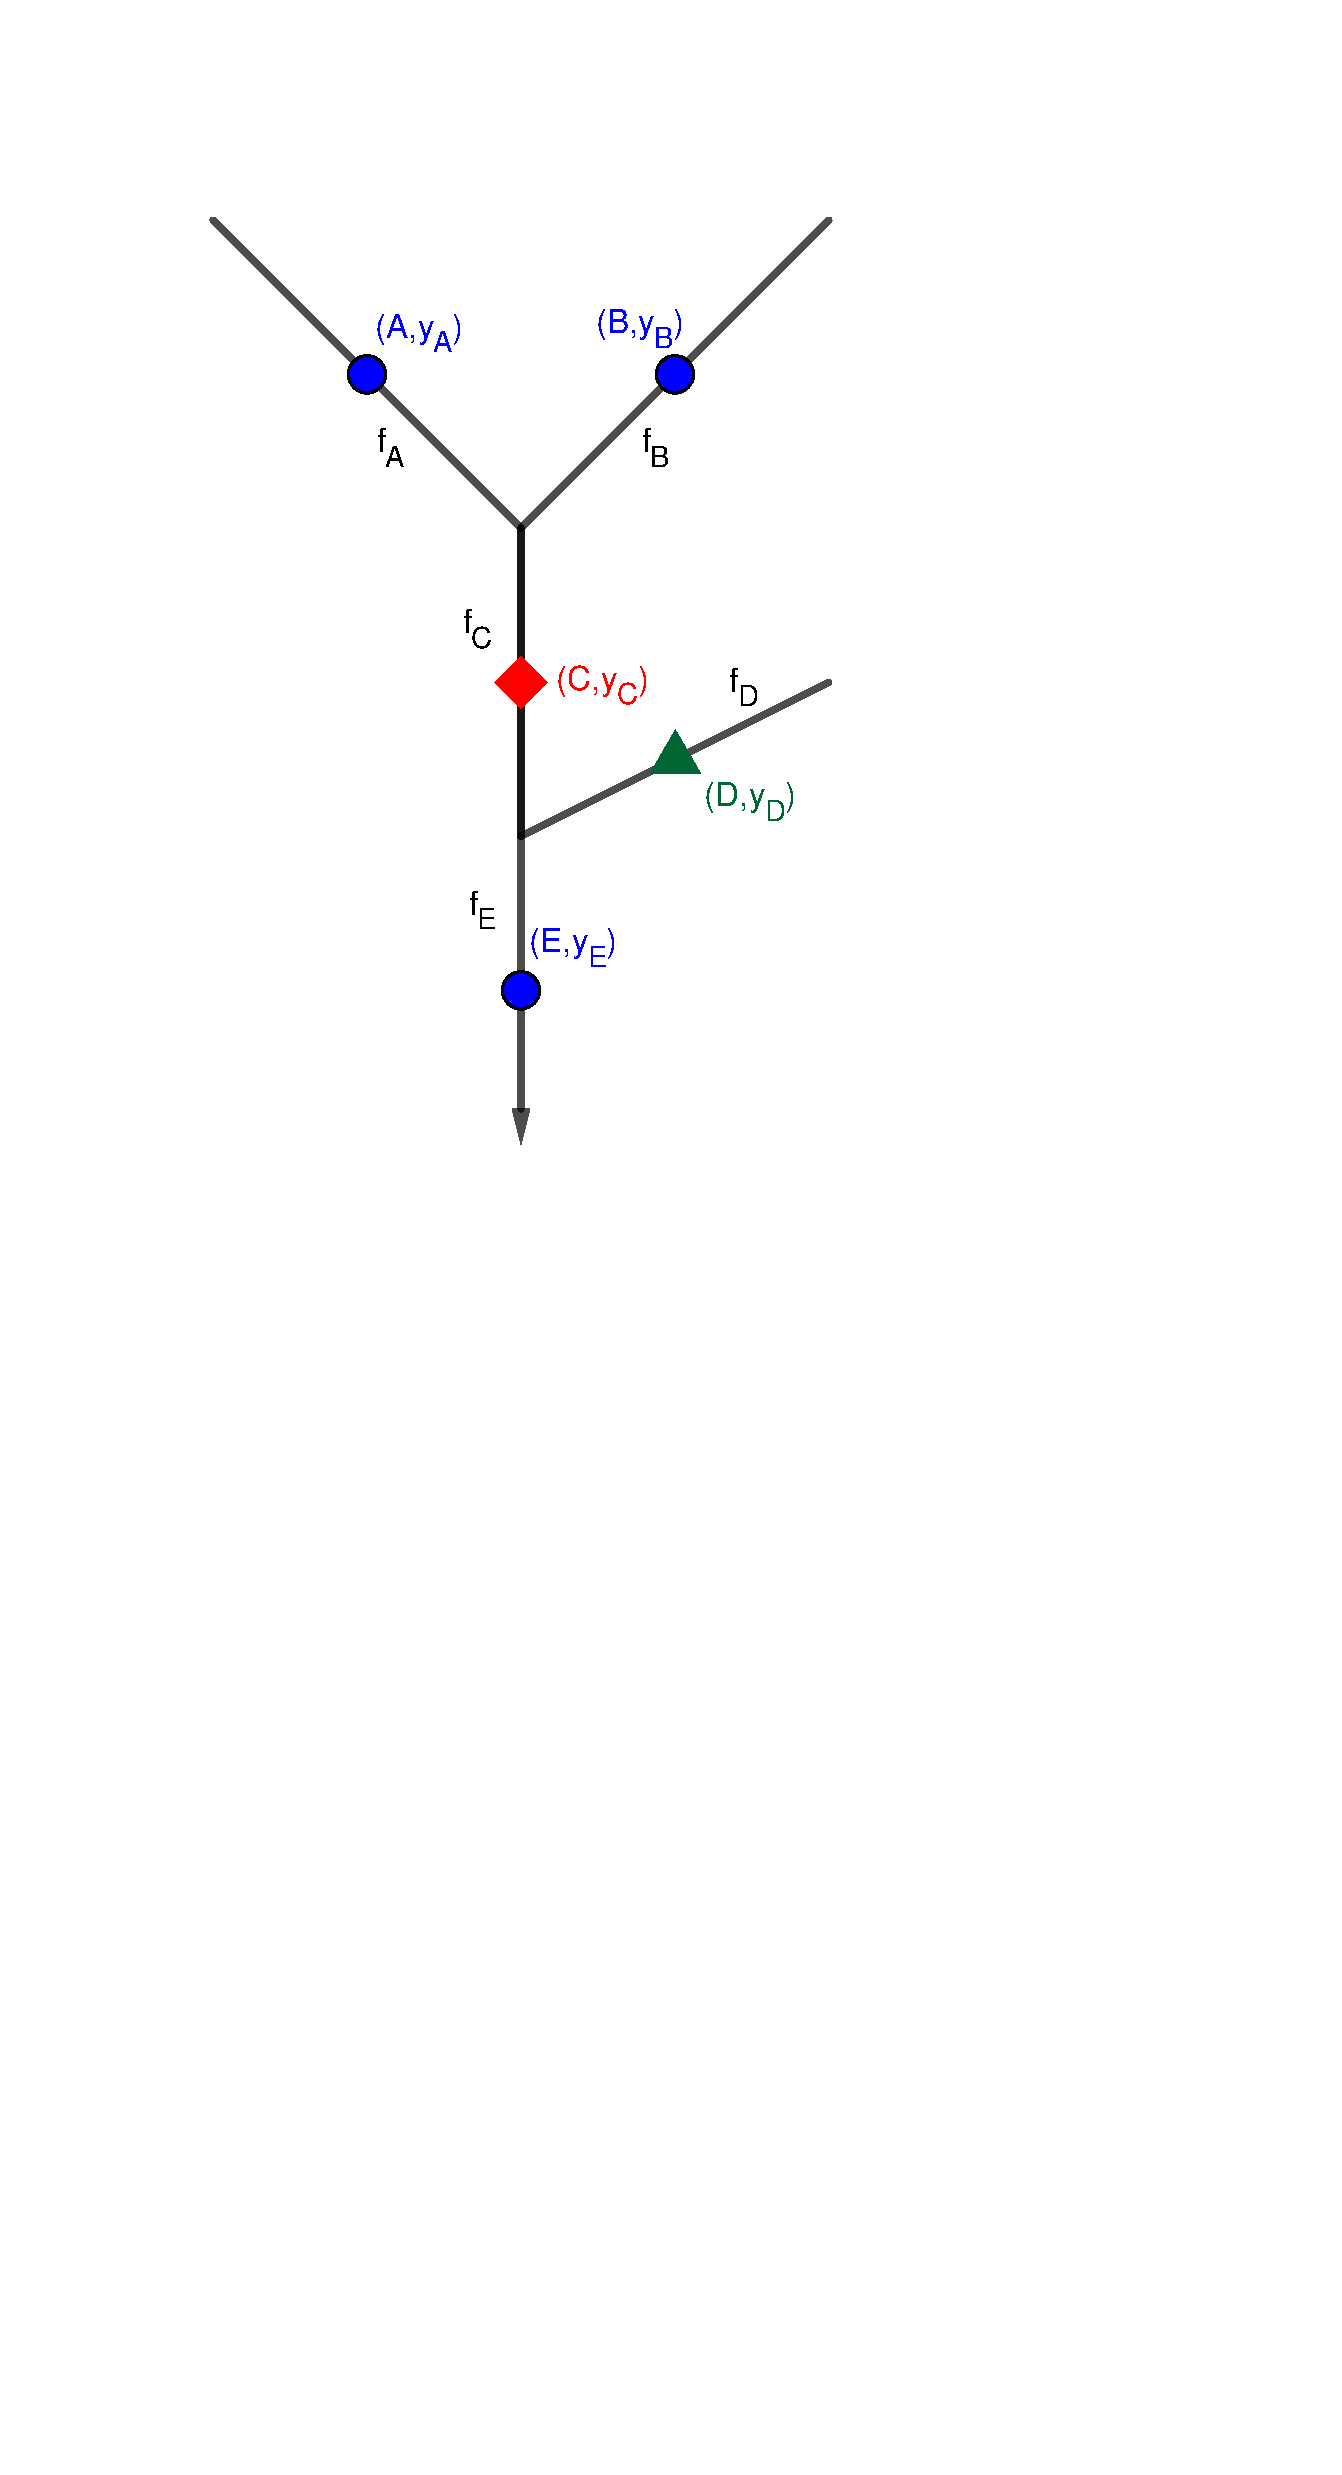
\includegraphics[width=0.35\textwidth]{Stream_result/Node-flow-complexed2-3.pdf}
	\vspace{-0mm}
	\caption{A simple example of streamflow data. Five solid black lines represent stream segments, indexed by $A,B,C,D,$ and $E$. Each line segment has its flow volume, called $f_{A}, f_{B}, \ldots, f_E$. $y_{A}, \ldots , y_{E}$ denote water quality values of each segment.}
	\label{fig:nodedescription}
\end{figure}

We consider a toy example network shown in Figure \ref{fig:nodedescription}. Suppose that there are five observation points ($A$, $B$, $C$, $D$, $E$) in the different stream segments of a river network. Assume that each segment has a flow volume of $f$. Let $f_A, f_B, \ldots, f_E$ denote the flow volume of station $A, B,\ldots, E$, respectively. We further denote $y_A, y_B, \ldots, y_E$ as water quality observations at station $A, B, \ldots, E$, respectively.

\subsection{Neighborhood selection}\label{subsec:nbd}

The concept of ``flow-connected" introduced in \cite{VerHoef(2006)} is useful to build a neighborhood set of a point in a river network. \cite{VerHoef(2006)} defined that two locations are connected when the intersection of upstreams of two stations is a non-empty set. In our example, segments $A, C$ and $B, C$ are ``flow-connected'' because the water in $A$ and $B$ can go to location $C$. On the other hand, $C$ and $D$ are not flow-connected since the water in $C$ cannot go to station $D$ or vice versa. 

We use the concept of ``flow-connected'' to determine whether the two segments are neighbors or not. In this study, when two points are flow-connected, we consider each other neighbors. In Figure \ref{fig:nodedescription}, suppose that we are interested in removing point $C$ at a specific resolution level. By following the concept of flow-connected, $A, B$, and $E$ (blue circles) are defined as its neighbors, and $D$ (green triangle) is excluded from the neighborhood of $C$.

One of the distinct characteristics of the proposed neighborhood selection is that it considers both upstream and downstream neighborhoods. By doing so, it can reduce the number of boundary points. At first glance, including downstream points into the neighborhood seems awkward. However, by combining an appropriate prediction filter construction explained in Section \ref{subsec:pf}, it can generate reasonable prediction filters.

\subsection{Construction of prediction filter }\label{subsec:pf}

In this section, we consider the problem of the prediction filter construction. The simplest prediction filter is constructed using an equally weighted value vector. However, every river network has its mainstream and sub-streams. It is plausible that observations on the mainstream usually have a stronger effect on nearby observations. Therefore, the effect of each stream on  a given segment should be different. To take into account the influence of each stream segment, we use flow volumes. For the construction of the prediction filter, we consider the size of flow volumes compared to others, called ``relative flow volumes" \citep{ODonnell2014}.

Suppose that we have neighbors of a specific point in a river network. An easy way to weigh is to give the same weight to all neighbors, which may not be desirable. For example, if $f_A$ is much larger than $f_B$, $y_A$ has a more significant effect on $y_C$ than $y_B$. Also, if $f_D$ is larger than $f_C$, $y_E$ is much different from $y_C$. Therefore, we intend to construct flow-adaptive weights that reflect the above considerations. 
We now consider predicting the response value of point $C$ with the neighbors in the toy example in Figure \ref{fig:nodedescription}. Since $f_{C}= f_{A}+ f_{B}$, flow-adaptive weights for point $C$ can be defined as ratios of flows, 
\begin{equation}
w_{A} = \frac{f_{A}}{f_{C}},~~w_{B}=\frac{f_{B}}{f_{C}}, ~\text{ and }~ w_{E}=\frac{f_{C}}{f_{E}}.
\label{eqn:flowadaptiveweight}
\end{equation}
Then we obtain a predicted value of $y_{C}$ as $\hat{y}_{C} = \tilde{w}_{A}y_{A} + \tilde{w}_{B}y_{B} + \tilde{w}_{E}y_{E},$  where
\begin{align}
\tilde{w}_{A} &= \frac{f_{A}/f_{C}}{f_{A}/f_{C} + f_{B}/f_{C} + f_{C}/f_{E}},\nonumber\\
\tilde{w}_{B} &= \frac{f_{B}/f_{C}}{f_{A}/f_{C} + f_{B}/f_{C} + f_{C}/f_{E}}, \text{ and } \label{eqn:streamliftingweight}\\
\tilde{w}_{E} &= \frac{f_{C}/f_{E}}{f_{A}/f_{C} + f_{B}/f_{C} + f_{C}/f_{E}},\nonumber
\end{align}
which are normalized flow-adaptive weights to make the sum of weights to be 1, i.e., $\tilde{w}_A + \tilde{w}_B + \tilde{w}_E = 1$. Therefore, the predicted value of the segment $C$, $\hat{y}_{C}$ is
\[
\hat{y}_{C}  = \tilde{w}_{A}y_{A} + \tilde{w}_{B}y_{B} + \tilde{w}_{E}y_{E}.
\]

Hence, we provide a lifting scheme for streamflow data by combining flow-adaptive weights of (\ref{eqn:flowadaptiveweight}) and (\ref{eqn:streamliftingweight}) with the conventional lifting scheme. In practice, it is rare to know all $f$ values on the entire streamlines. Therefore, it is necessary to estimate flow values. For example, \cite{VerHoef(2006)} used equal weights for each split. In this study, it is assumed that the flow volume $f$ in most upstream segments is proportional to their stream order and segment length. Note that the stream order is a positive whole number that is often used in hydrology to define stream-based distance in river networks. There are several stream orders. Among them, the Shreve stream order is one of the most straightforward stream orders \citep{Cressie2006, VerHoef(2010)}. \cite{Cressie2006} defined the stream order as the number of sources in the upstream portion of the river network. The Shreve stream order starts from setting all most upstream segments to 1. Magnitudes increase at all junctions in the river network. For example, if a stream has a magnitude one and combines with a new stream having magnitude 2, it becomes magnitude 3. By doing so, it is able to configure all magnitudes of the given network.

To approximate $f$ values, we use the Shreve stream order and assume that the flow of the most upstream segments is  proportional to their lengths to prevent multiple tie values of flow volumes. After defining flow volumes of most upstream segments, one can define flow volumes of the next upstream segments as a sum of their upstream segments. By repeating this approach, we obtain all $f$ values in the river network. It is also assumed that the weights associated with the flow volumes are known to generate $\log(\sqrt{f})$ values. Following \cite{ODonnell2014}, we normalize the $\log(\sqrt{f})$ values, which are  between $0.2$ to $1.5$.
			
\subsection{Removal point selection}

The removal order should be determined for the streamflow lifting scheme. If the data lie in the real line, it is easy to apply the conventional approach, such as  \cite{Nunes2006}. They used the length of points on the real line for integral calculations. Moreover, it can be extended to the two-dimensional data proposed by \cite{Jansen2009}. To determine the removal point, \cite{Jansen2009} found the highest density observation in the Euclidean domain by considering the integral of the scaling function. In addition, they proposed measuring the Voronoi-polygon based area as a candidate for proper integrals and chose to have the smallest integration point as a removal point in the LOCAAT algorithm.

However, these methods cannot be applied directly to streamflow data because the network is not easily projected into one- or two-dimensional data. In the streamflow lifting scheme, a simple approach is proposed to measure the contribution of each segment in the data to distinguish the points located in the most densest areas of the river network. We define an integral as the contribution of each observation point to the network. More specifically, to define the contribution of each point in streamflow data, we use flow-adaptive weights defined in (\ref{eqn:streamliftingweight}). A simple example is illustrated in Figure \ref{fig:nodedescription}. Suppose that at the $j$th level, we want to remove point $C$ with neighborhood points $A, B$, and $E$. Let $I_A^{j}$ denote the integral of point $A$ at the $j$th level, which is defined by the volume of the segment where $A$ is located, say $V_A$,
\begin{align*}
I_A^{j} &= V_A = f_A\times \ell_A,\nonumber\\
I_B^{j} &= V_B = f_B\times \ell_B, \text{ and }\\
I_E^{j} &= V_E = f_E\times \ell_E.\nonumber
\end{align*}
At the next level $j-1$ after point $C$ is removed, we need to update the integral of neighborhood points. For this purpose, we use a weighted volume of the point $C$ according to the weights of neighbors in (\ref{eqn:streamliftingweight}). Thus, $I_A^{j}, I_{B}^{j},$ and $I_E^{j}$ are updated to
\begin{align*}
I_A^{j-1}&=I_A^{j} + \tilde{w}_A\times V_C,\nonumber\\
I_B^{j-1}&= I_B^{j} + \tilde{w}_B \times V_C, \text{ and }\\
I_E^{j-1} &= I_E^{j} + \tilde{w}_E \times V_C.\nonumber
\end{align*}
Note that since $\tilde{w}_A\times V_C +\tilde{w}_B \times V_C+ \tilde{w}_E \times V_C=I_C^{j}$, the sum of integrals does not  change. We select a point that has the minimum value of $I^{j-1}$ for the removal point at the $j-1$th level. For the update filter, we use the minimum norm solution-based filter in (\ref{eqn:updatefilter}).

\subsection{Nondecimated lifting scheme for streamflow data}

In this section, the proposed lifting scheme is generalized to a nondecimated version of the streamflow lifting scheme that can  reduce the mean squared error of the lifting scheme in nonparametric regression settings, as mentioned in Section \ref{subsec:otherlifting}. For this purpose, we assume that the current stream distance-based removal order is one of the well-behaved trajectories in terms of the root mean squared error. Then we generate multiple trajectories from permutations. To generate these well-behaved trajectories, we first make clusters of observations and do permutation to those within the same cluster. For implementation, two tuning parameters should be used: (i) the number of trajectories (\texttt{Q=10}) and (ii) the number of permutation within a single trajectory (\texttt{v=5}). %Note that we can have the same denoising results when we use \texttt{Q=10} and \texttt{v=0}.

\section{Simulation study}\label{sec:streamflowsimulationdata}

This section conducts numerical experiments for the evaluation of our approach for streamflow data analysis. Assume that the data are observed from the regression model of \ref{eq:scattered}. We mainly focus on the situation in which the underlying mean-field of the data is piecewise constant. Thus, there are several discontinuous function values in a river network, which may not be able to make proper estimates using conventional smoothing-based methods. For comparison, we consider the flexible smoothing approach of \cite{ODonnell2014} and three variants of the proposed method: streamflow lifting scheme with median thresholding (\texttt{S-Lifting (M)}), streamflow lifting scheme with hard thresholding (\texttt{S-Lifting (H)}), and nondecimated streamflow lifting scheme with median thresholding (\texttt{S-Lifting (N)}).

\begin{figure}
	\centering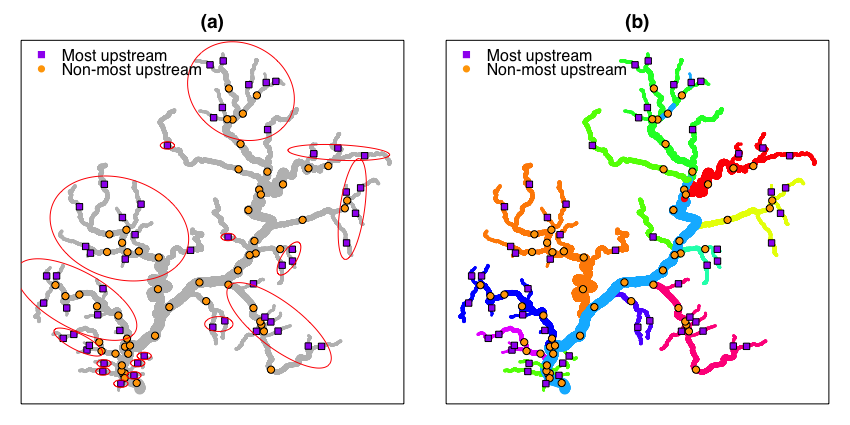
\includegraphics[width=1\textwidth]{Stream_result/Stream_cluster_maps_new(5).png}
	\centering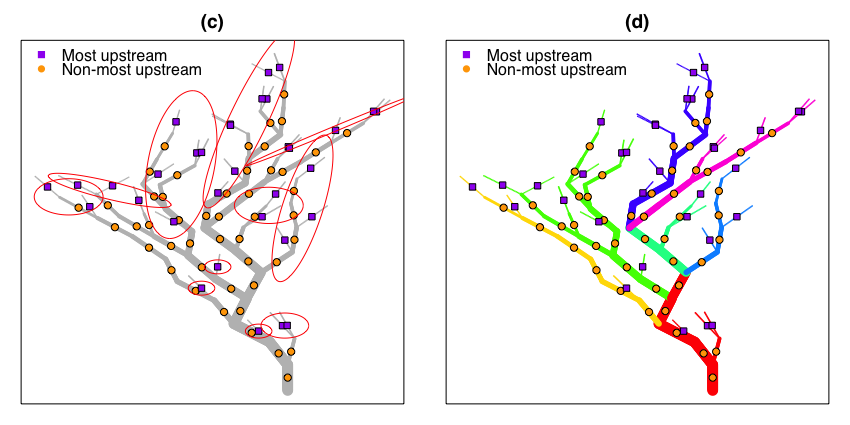
\includegraphics[width=1\textwidth]{Stream_result/Stream_cluster_maps_STPCA(2).png}
	\vspace{-10mm}\caption{(a) Clusters (red circles) in the Miho-Cheon stream network. Note that the most upstream segments (purple squares) and the non-most upstream segments (orange circles). (b) Colors represent sub-streams for the sampling procedure. The sampling probability is proportional to the number of streams of each sub-stream. {\color{red} (c) and (d) show the same information of (a) and (b) for simulated river network used in \cite{Gallacher2017}.}} 
	\label{fig:clusterconstruction}
\end{figure}

For simulation setup, two types of river networks are considered: one is the Miho-Cheon streamflow segments in Figure \ref{fig:clusterconstruction}(a) and (b), and the other is the simulated river network in Figure \ref{fig:clusterconstruction}(c) and (d), which was used in \cite{Gallacher2017}. The two networks consist of 113 stream segments and 80 stream segments, respectively. For each river network, the entire stream segments are divided into two groups: most upstream segments and non-most upstream segments, as shown in Figure \ref{fig:clusterconstruction} (a). Assume that there are no intrinsic sources to change the simulated signal values. The signal values in the non-most upstream segments are then generated from a weighted average of nearby upstream signal values. It implies that the simulation is sufficient to generate only the signal values in the most upstream segments. 

In addition, we divide the most upstream segments into several clusters, as shown in red circles Figure \ref{fig:clusterconstruction} (a) and (c), to generate inhomogeneous stream network data. We assume that the signal values for all most upstream segments within the cluster are the same. For each simulated data set, $g(x_i)$ values of the most upstream segments are generated as follows: (i) All $g(x_i)$ values in the most upstream segments are set to be 9. (ii) A cluster is randomly selected from the clusters in Figure  \ref{fig:clusterconstruction}, and (iii) $g(x_i)$ values in the selected cluster are replaced with a value that is randomly chosen from $\{12, 15, 18\}$. This procedure is repeated until at least 30 most upstream segments have values greater than 9. A realization of the simulated data generation is shown in Figure \ref{fig:streamsimresult} (a) and Figure \ref{fig:streamsimresult2} (a).

Three spatial sampling designs are also considered for simulation data in river networks. (i) For a sparse design, among a total of 113 Miho-Cheon stream segments, 40 stations located on 40 different segments are considered. A realization is shown in Figure \ref{fig:clusterconstruction}(b). (ii) 80 stations are used, which is nearly two-thirds of the number of the Miho-Cheon streams. (iii) 113 stations are considered as a dense case. Along the same line, we analyze the simulated network of \cite{Gallacher2017} in two designs: (i) observations are generated at 40 stations, and (ii) one observation is simulated in each segment. 
\textcolor{red}{To selects stations in a river network, we use a spatial stratified sampling approach to make the resulting stations are evenly distributed in the network. Groups used in the sampling procedure are shown in Figure (b) and (d), respectively.} 

The noise terms are generated from $\varepsilon_{i} \stackrel{\text{i.i.d.}}{\sim} \mathcal{N}(0,\sigma^{2})$ with $\sigma=0.5$,  $\sigma=1$, and $\sigma=1.5$. As for the evaluation measure, we consider the root mean square error (RMSE) as 
%\begin{equation}\label{eq:RMSE}
\[
\text{RMSE}=\sqrt{\frac{\sum_{i=1}^{N_{tot}} (g(x_i)-\hat{g}(x_i))^{2}} {N_{tot}}},
\]
%\end{equation}
where $\hat{g}(x_i)$ is an estimate of segment $i$, and $N_{tot}$ denotes the total number of stream segments in the river network. For each combination of three spatial designs and three $\sigma$'s, we compute RMSE values according to our methods and the approach of \cite{ODonnell2014} over 100 simulated data sets. 

Tables \ref{table:streamsimresult} and \ref{table:streamsimresult2} list the averages of RMSE values under the two river networks. From results in the tables, we have some observations: (i) The proposed method outperforms the approach of \cite{ODonnell2014} for most of the combinations. (ii) The proposed methods work well under the given simulation settings, especially when $\sigma$ is small. (iii) The method by \cite{ODonnell2014} provides stable results across the number of sampling observations and $\sigma$'s, while the performance of the proposed methods is affected by both scenarios. (iv) The nondecimated version of the proposed lifting scheme is well performed in most cases. 
For visual inspection, we look at one realization example of the fitting results of the spatial design with 60 stations and $\sigma=1$ shown in Figures \ref{fig:streamsimresult} and \ref{fig:streamsimresult2}. It seems that the proposed methods are well performed, reflecting the inhomogeneous features of the underlying fields in the two river networks.   

We finally note that R codes used to implement the methods and to carry out some experiments are available at \url{https://github.com/SeoncheolPark/paper_StreamflowLifting/tree/master/code} in order that one can reproduce the same results. 

\begin{table}[]
	\centering
	\caption{Averages of RMSE values (standard error) over 100 simulations.}
	\resizebox{\textwidth}{!}{\begin{tabular}{|c|c|c|c|c|c|c|c|c|c|}
			\hline
			\multirow{2}{*}{\begin{tabular}[c]{@{}c@{}}RMSE\\ (Std. error)\end{tabular}} & \multicolumn{3}{c|}{Obs=40}          & \multicolumn{3}{c|}{Obs=80}    & \multicolumn{3}{c|}{Obs=113}              \\ \cline{2-10} 
			& $\sigma=1$                                                         & $\sigma=1.5$                                                       & $\sigma=2$                                                         & $\sigma=1$                                                         & $\sigma=1.5$                                                       & $\sigma=2$                                                         & $\sigma=1$                                                         & $\sigma=1.5$                                                       & $\sigma=2$                                                         \\ \hline
			O'Donnell                                                                    & \begin{tabular}[c]{@{}c@{}}2.0988\\ (0.1957)\end{tabular}          & \begin{tabular}[c]{@{}c@{}}2.2101\\ (0.2052)\end{tabular}          & \textbf{\begin{tabular}[c]{@{}c@{}}2.2882\\ (0.2317)\end{tabular}} & \begin{tabular}[c]{@{}c@{}}1.5270\\ (0.1561)\end{tabular}          & \begin{tabular}[c]{@{}c@{}}1.6336\\ (0.1513)\end{tabular}          & \begin{tabular}[c]{@{}c@{}}1.7542\\ (0.1654)\end{tabular}          & \begin{tabular}[c]{@{}c@{}}1.3252\\ (0.1364)\end{tabular}          & \begin{tabular}[c]{@{}c@{}}1.4458\\ (0.1320)\end{tabular}          & \begin{tabular}[c]{@{}c@{}}1.5798\\ (0.1609)\end{tabular}          \\ \hline
			\begin{tabular}[c]{@{}c@{}}Proposed\\ (Median)\end{tabular}                  & \begin{tabular}[c]{@{}c@{}}1.7089\\ (0.4181)\end{tabular}          & \begin{tabular}[c]{@{}c@{}}2.1410\\ (0.5202)\end{tabular}          & \begin{tabular}[c]{@{}c@{}}2.3588\\ (0.5134)\end{tabular}          & \begin{tabular}[c]{@{}c@{}}1.0662\\ (0.1877)\end{tabular}          & \begin{tabular}[c]{@{}c@{}}1.3488\\ (0.2343)\end{tabular} & \begin{tabular}[c]{@{}c@{}}1.6377\\ (0.2686)\end{tabular} & \begin{tabular}[c]{@{}c@{}}0.8362\\ (0.1187)\end{tabular} & \begin{tabular}[c]{@{}c@{}}1.1656\\ (0.1929)\end{tabular} & \begin{tabular}[c]{@{}c@{}}1.4141\\ (0.2119)\end{tabular} \\ \hline
			\begin{tabular}[c]{@{}c@{}}Proposed\\ (Hard)\end{tabular}                    & \textbf{\begin{tabular}[c]{@{}c@{}}1.6287\\ (0.3882)\end{tabular}} &
			\begin{tabular}[c]{@{}c@{}}2.1281\\ (0.4913)\end{tabular} & \begin{tabular}[c]{@{}c@{}}2.3647\\ (0.4704)\end{tabular}          & \textbf{\begin{tabular}[c]{@{}c@{}}1.0382\\ (0.1528)\end{tabular}} & \begin{tabular}[c]{@{}c@{}}1.3440\\ (0.1903)\end{tabular}          & \begin{tabular}[c]{@{}c@{}}1.6400\\ (0.2524)\end{tabular}          & \begin{tabular}[c]{@{}c@{}}0.8386\\ (0.1074)\end{tabular}          & \begin{tabular}[c]{@{}c@{}}1.2142\\ (0.1569)\end{tabular}          & \begin{tabular}[c]{@{}c@{}}1.5172\\ (0.1985)\end{tabular}          \\ \hline
			\begin{tabular}[c]{@{}c@{}}Proposed\\ (Median, nlt)\end{tabular}                    & \begin{tabular}[c]{@{}c@{}}1.7210\\ (0.3907)\end{tabular} & \textbf{\begin{tabular}[c]{@{}c@{}}2.1143\\ (0.4517)\end{tabular}} & \begin{tabular}[c]{@{}c@{}}2.3292\\ (0.4460)\end{tabular}          & \begin{tabular}[c]{@{}c@{}}1.0428\\ (0.1849)\end{tabular}  & \textbf{\begin{tabular}[c]{@{}c@{}}1.3212\\ (0.2241)\end{tabular}}          & \textbf{\begin{tabular}[c]{@{}c@{}}1.6076\\ (0.2588)\end{tabular}}          & \textbf{\begin{tabular}[c]{@{}c@{}}0.8000\\ (0.1158)\end{tabular}}          & \textbf{\begin{tabular}[c]{@{}c@{}}1.1225\\ (0.1760)\end{tabular}}          & \textbf{\begin{tabular}[c]{@{}c@{}}1.3705\\ (0.2081)\end{tabular}}          \\ \hline
	\end{tabular}}
	\label{table:streamsimresult}
\end{table}
	\vspace{-1mm}


\begin{figure}
	\centering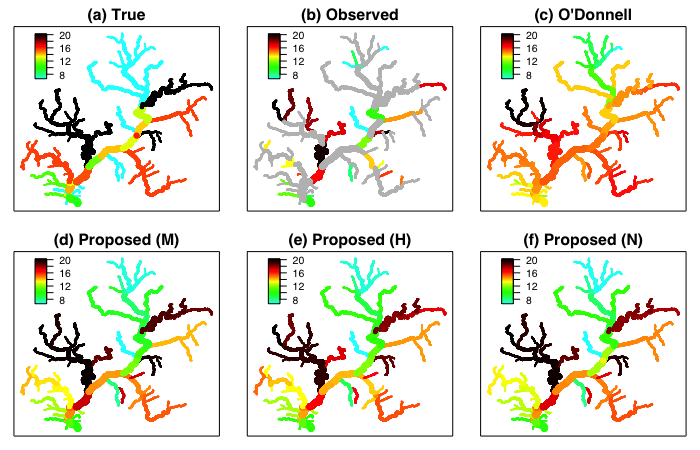
\includegraphics[width=0.95\textwidth]{Stream_Result/SLifting_Comp_02.png}
	\vspace{-4mm}\caption{(a) True signal, (b) noisy observations when $\text{Obs=40}$ \textcolor{red}{with unobserved segments shown in gray lines}, (c) fit by \cite{ODonnell2014}, (d)-(e) fits by the proposed method with median thresholding and hard thresholding, and (f) fit by the proposed nondecimated method with median thresholding.}
	\label{fig:streamsimresult}
\end{figure}


\begin{figure}
	\centering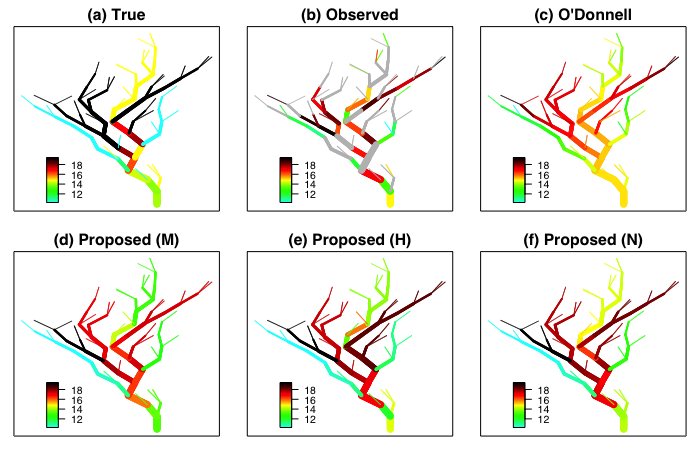
\includegraphics[width=0.95\textwidth]{Stream_Result/SLifting_Comp_03.png}
	\vspace{-4mm}\caption{(a) True signal, (b) noisy observations when $\text{Obs=60}$ \textcolor{red}{with unobserved segments shown in gray lines}, (c) fit by \cite{ODonnell2014}, (d)-(e) fits by the proposed method with median thresholding and hard thresholding, and (f) fit by the proposed nondecimated method with median thresholding.}
	\label{fig:streamsimresult2}
\end{figure}


\begin{table}[]
	\centering
	\caption{Averages of RMSE values of streamflow data used in \cite{Gallacher2017} (standard errors) over 100 simulations.}
	{\footnotesize
	\resizebox{\textwidth}{!}{\begin{tabular}{|c|c|c|c|c|c|c|}
			\hline
			\multirow{2}{*}{\begin{tabular}[c]{@{}c@{}}RMSE\\ (Std. error)\end{tabular}} & \multicolumn{3}{c|}{Obs=40}            & \multicolumn{3}{c|}{Obs=80}            \\ \cline{2-7} 
			& $\sigma=1$                                                         & $\sigma=1.5$                                                       & $\sigma=2$                                                         & $\sigma=1$                                                         & $\sigma=1.5$                                                       & $\sigma=2$                                                         \\ \hline
			O'Donnell                                                                    & \begin{tabular}[c]{@{}c@{}}1.7266\\ (0.2638)\end{tabular}          & \begin{tabular}[c]{@{}c@{}}1.8695\\ (0.2835)\end{tabular}          & \begin{tabular}[c]{@{}c@{}}1.9698\\ (0.2839)\end{tabular}          & \begin{tabular}[c]{@{}c@{}}1.2698\\ (0.1251)\end{tabular}          & \begin{tabular}[c]{@{}c@{}}1.3815\\ (0.1727)\end{tabular}          & \begin{tabular}[c]{@{}c@{}}1.5421\\ (0.2017)\end{tabular}          \\ \hline
			\begin{tabular}[c]{@{}c@{}}Proposed\\ (Median)\end{tabular}                  & \begin{tabular}[c]{@{}c@{}}1.1716\\ (0.2530)\end{tabular}          & \begin{tabular}[c]{@{}c@{}}1.5464\\ (0.3611)\end{tabular} & \begin{tabular}[c]{@{}c@{}}1.8121\\ (0.3539)\end{tabular} & \begin{tabular}[c]{@{}c@{}}0.7265\\ (0.1212)\end{tabular}          & \begin{tabular}[c]{@{}c@{}}1.0249\\ (0.1510)\end{tabular} & \begin{tabular}[c]{@{}c@{}}1.2818\\ (0.2599)\end{tabular} \\ \hline
			\begin{tabular}[c]{@{}c@{}}Proposed\\ (Hard)\end{tabular}                    &\textbf{\begin{tabular}[c]{@{}c@{}}1.1417\\ (0.2244)\end{tabular}} & \begin{tabular}[c]{@{}c@{}}1.5769\\ (0.3050)\end{tabular}          & \begin{tabular}[c]{@{}c@{}}1.9040\\ (0.3286)\end{tabular}          & \begin{tabular}[c]{@{}c@{}}0.7396\\ (0.1317)\end{tabular} & \begin{tabular}[c]{@{}c@{}}1.0666\\ (0.1678)\end{tabular}          & \begin{tabular}[c]{@{}c@{}}1.3705\\ (0.2495)\end{tabular}          \\ \hline
			\begin{tabular}[c]{@{}c@{}}Proposed\\ (Median, nlt)\end{tabular}                    & \begin{tabular}[c]{@{}c@{}}1.1443\\ (0.2494)\end{tabular}          & \textbf{\begin{tabular}[c]{@{}c@{}}1.4988\\ (0.3267)\end{tabular}}          & \textbf{\begin{tabular}[c]{@{}c@{}}1.7329\\ (0.3385)\end{tabular}}          & \textbf{\begin{tabular}[c]{@{}c@{}}0.7162\\ (0.1219)\end{tabular}} & \textbf{\begin{tabular}[c]{@{}c@{}}1.0106\\ (0.1678)\end{tabular}}          & \textbf{\begin{tabular}[c]{@{}c@{}}1.2816\\ (0.2712)\end{tabular}}          \\ \hline
	\end{tabular}}
	\label{table:streamsimresult2}}
	\vspace{-1mm}
\end{table}


\section{Real data analysis}\label{sec:streamflowrealdata}
In this section, we apply the proposed lifting scheme to the real data set in Section \ref{sec:data}. We consider the TOC water pollutant observed from 2012 to 2017. Water pollutants typically have some extreme values, which results in skewed empirical distributions. Therefore, we consider the average values of the log transformation of TOC data from 2012 to 2017 at each station shown in Figure \ref{fig:fig1}.
For the configuration of the results, we use an interpolation method based on equation (\ref{eqn:streamliftingweight}). We consider the river network in Figure \ref{fig:nodedescription}. Suppose that there are no observations in segment $C$. That is, we assume that the actual value of $y_c$ is unknown. Then we interpolate the value of $y_c$ with observations $y_A, y_B$, and $y_E$, which results in $\hat{y}_{C} = w_{A}y_A + w_{B}y_B + w_{E}y_E$, where $w_{A} + w_{B} + w_{E} = 1$. 
For the nondecimated version of the streamflow lifting scheme, clusters should be set up to achieve stable smoothing results.  In this analysis, we only consider a permutation of observations in the same stream segments, assuming that the original removal path defined through Section \ref{sec:streamflowliftingscheme} is such a well-behaved removal order. Twelve of the 127 stations are located in segments with two or more stations.

Assume that the underlying model of TOC data follows the model of {\color{blue}(\ref{eqn:spatialsimpleadditive})}. Although the actual function $g$ is unknown, the similarity of interpolation can be evaluated by the approximated root mean square error ($\widetilde{\text{RMSE}}$),
\[
\widetilde{\text{RMSE}}=\sqrt{\frac{\sum_{i=1}^{N_{tot}} (\tilde{g}(x_i)-\hat{g}(x_i))^{2}} {N_{tot}}},
\]
where $N_{tot}=942$ is the total number of stream segments in the Geum-River network, $\tilde{g}(x_i)$ denote the interpolation of raw data, and $\hat{g}(x_i)$ represents the interpolation of estimates. 

\begin{figure}
	\centering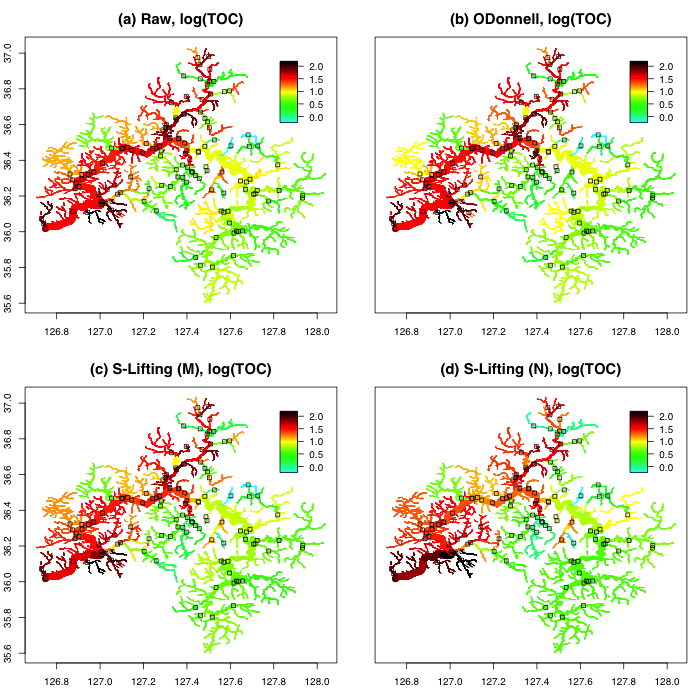
\includegraphics[width=0.95\textwidth]{Stream_result/result_TOC3.png}
	\vspace{-3mm}
	\caption{Real data analysis for TOC data.  (a) Interpolation of row dataset, (b) interpolation of estimates by O'Donnell's method, (c) interpolation of estimates by the proposed streamflow lifting scheme with median thresholding, and (d) interpolation of estimates by the proposed nondecimated streamflow lifting scheme with median thresholding.}
	\label{fig:realanalysis}
\end{figure}

Figure \ref{fig:realanalysis} shows the results by the proposed streamflow lifting scheme for the Miho-Cheon TOC data set. The interpolation for raw data is shown in panel (a). For comparison, we consider the method of \cite{ODonnell2014}. Its results are shown in panel (b). The interpolation results of the proposed methods are in panels (c) and (d), respectively. The nondecimated lifting scheme uses a bunch of random trajectories so that the results can vary over executions. From Figure \ref{fig:realanalysis}, we observe that the high TOC values of the Geum-River downstream are affected by the water quality of the Miho-Cheon. In other words, TOC from the Miho-Cheon dominates the water pollution in the Geum-River downstream. As for Figure \ref{fig:studyarea}, we find that many industrial factories are near the Miho-Cheon catchment area. It is a plausible conclusion that industrial factories can affect the amount of TOC in the river network.

\begin{table}[]
	\centering
	\caption{$\widetilde{\text{RMSE}}$ results of the interpolation of the Geum-River data set.}
	\begin{tabular}{|c|c|c|c|}
		\hline
		& ODonnell & S-Lifting (M) & S-Lifting (N) \\ \hline
		$\widetilde{\text{RMSE}}$ & 0.1240   & 0.0818        & 0.1856        \\ \hline
	\end{tabular}
	\label{table:realanalysis}
\end{table}

In addition, from Figure \ref{fig:realanalysis}, all methods present smoothed results compared to the representation of the raw data. The proposed streamflow lifting schemes in panels (c) and (d) provide more smoothed estimation results. From panels (b) and (c), we observe that the O'Donnell's approach yields some orange colors on the Eastside while these colors are changed to green colors in the proposed streamflow lifting scheme. {\color{red}Moreover, the proposed lifting scheme decides some yellow values of the Westside on the network are noises. Therefore, the method also changes it into orange or red.}

For the result of the nondecimated version, we find that some values on the east side of the network are high. The real data seems to be a mixed pattern instead of a piecewise function. So, it is challenging to establish appropriate clusters to carry out  the nondecimated streamflow lifting scheme. Compared to this result, the original streamflow lifting scheme and the approach of \cite{ODonnell2014} give more robust results. This observation is supported by the results of  $\widetilde{\text{RMSE}}$ values listed in Table \ref{table:realanalysis}. 

\begin{figure}
	\centering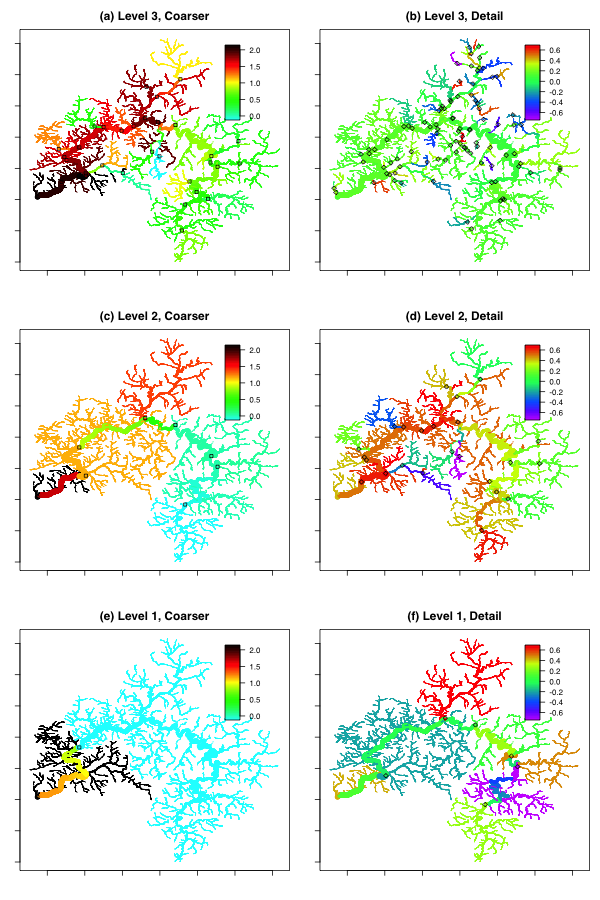
\includegraphics[width=0.85\textwidth]{Stream_result/result_TOC_detail3(rev).png}
	\vspace{-2mm}
	\caption{A multiscale analysis of TOC data. (a), (c) and (e) show global components of streamflow data at three different levels.  (b), (d)  and (f) are corresponding detail components. The number of points at each level (\texttt{nkeep}) are \texttt{32, 8, 2,} respectively.}
	\label{fig:resultBODdetail}
\end{figure}

Before closing this section, we perform a multiscale analysis of streamflow data, which is one of the advantages of the proposed streamflow lifting scheme method. Let $g_4(x)$ be a representation at the finest level. We then decompose the function $g_4(x)$ into global component $g_3(x)$ and detailed component $d_3(x)$. It further breaks down the function $g_3(x)$ into global component $g_2(x)$ and detailed component $d_1(x)$.  By repeating the above steps until a certain level $1$, we finally decompose the $g_4(x)$ as
\[
g_4(x)=g_1(x)+\sum_{\ell=1}^{3}d_\ell(x), 
\]
where $\ell$ denotes the resolution index. As $\ell$ decreases, the corresponding representation becomes coarser. To perform this multiscale analysis of the TOC data in the Geum-River network, we consider the representation in Figure \ref{fig:realanalysis}(c) as the finest level representation $g_4(x)$. Figure \ref{fig:resultBODdetail} shows the multiscale representations by the proposed streamflow lifting scheme. In Figure \ref{fig:resultBODdetail}(a), we reconstruct the river network field only using 32 stations out of 127 stations, which still holds global features of the representation in Figure \ref{fig:realanalysis}(c). The difference between the two representations is shown in Figure \ref{fig:resultBODdetail}(a) as a detailed field. Figures \ref{fig:resultBODdetail}(c) and (e) show the global components of the representation in Figure \ref{fig:realanalysis}(c) using 8 stations and 2 stations, respectively, and  Figures \ref{fig:resultBODdetail}(d) and (f) show the corresponding differences. As the number of data points for reconstruction decreases, the corresponding representations are becoming rougher with focusing on global patterns. Instead, detail fields at each level provide some important information about networks that global components cannot represent.

\section{Concluding remarks}\label{sec:streamflowsummary}

In this paper, we have proposed a new lifting scheme for streamflow data. The proposed methods enable lifting scheme to streamflow data by (i) adopting a stream network adaptive neighborhood selection, (ii) constructing a prediction filter with flow-adaptive weighted averages, and (iii) setting a removal order by defining neighborhood flows of each observation point. By using the proposed neighborhood selection method, we reduce the number of boundary points and predict the values of upstream streamflow points. Besides, we have developed a nondecimated version of the proposed streamflow lifting scheme as a generalization. Simulation studies show that the proposed method works better than the conventional smoothing approach for streamflow data in particular situations, especially if there are some discontinuities in the data.

However, the proposed approach has some limitations. First, it is assumed that the volume of the water flow is proportional to the length of the segments and the Shreve order. In practice, however, the volume of the water flow may differ from the segment length and the Shreve order. The volume of the water varies over seasons. For example, precipitation in Korea is mostly is concentrated in the summer season. Second, in the simulation study, we have gathered segments in the given river network into several artificial groups to enhance the performance of the proposed lifting scheme. However, it is not easy to define optimal clusters in real data analysis. Therefore, one of the future studies will be to suggest an appropriate way to find optimal groups. Third, the removal order of the proposed method is not determined by the value of the streamflow data set, but based on location only. If possible, a data-adaptive removal order selection algorithm is useful to enhance the performance of the proposed method. %Finally, according to the arguments of \cite{Knight2009}, we have proposed a nondecimated version of the proposed streamflow lifting scheme, by assuming that there is no optimal removal order selection under the LOCAAT algorithm setting. It is reasonable to improve the performance with an optimal removal order. 

Finally, the approach proposed in this study does not provide spatio-temporal data analysis. Since TOC data are observed irregularly in both space and time domains, it is necessary to have a novel method to carry out spatio-temporal streamflow data analysis. \cite{Lindstrom2014} and \cite{ODonnell2014} solved this problem by calculating biweekly or monthly average data for each station. The method of \cite{ODonnell2014} can then be used to build space-time basis functions with tensor products. However, if we find a way to construct multiscale spatio-temporal bases without merging the data, it will be more useful to capture the multiscale spatio-temporal behavior of the data. It is reserved for future research.


\section*{Acknowledgement}
This research was supported by Basic Science Research Program through the National Research Foundation of Korea (NRF) funded by the Korea government (2018R1D1A1B07042933). The author Seoncheol Park would like to acknowledge that this research was undertaken thanks in part to funding from the Canada First Research Excellence Fund (Global Water Futures: Solutions to Water Threats in an Era of Global Change, Climate-Related Precipitation Extremes project), the Pacific Climate Impacts Consortium and the Canadian Statistical Sciences Institute.


%\section*{References}
\begin{thebibliography}{}

\bibitem[{Artiola {\it et al.}(2004)}]{Artiola2004}
Artiola, J, Pepper, I.~L., and Brusseau, M.~L. (2004). {\em Environmental Monitoring and Characterization}. Elsevier Science and Technology Books.

\bibitem[{Cressie {\it et al.}(2006)}]{Cressie2006}
Cressie, N., Frey, J., Harch, B., and Smith, M. (2006). Spatial prediction on a river network. {\em J. Agric. Biol. Environ. Stat.}, {\bf 11}, 127--150.

\bibitem[{Gallacher {\it et al.}(2017)}]{Gallacher2017}
Gallacher, K., Miller, C., Scott, E.~M., Willows, R., Pope, L., and Douglass, J. (2017). Flow-directed PCA for monitoring networks. {\em Environmetrics}, {\bf 28}, e2434. 

\bibitem[{Jansen and Oonincx (2005)}]{Jansen2005}
Jansen, M.~H., and Oonincx, P. (2005). {\em Second Generation Wavelets and Applications}. Springer Science and Business Media.

\bibitem[{Jansen {\it et al.}(2009)}]{Jansen2009}
Jansen, M., Nason, G.~P., and Silverman, B.~W. (2009). Multiscale methods for data on graphs and irregular multidimensional situations. {\em J. Roy. Stat. Soc. B.}, {\bf 71}, 97--125.

\bibitem[{Knight {\it et al.}(2009)}]{Knight2009}
Knight, M.~I., and Nason, G.~P. (2009). A `nondecimated' lifting transform. {\em Stat Comput.}, {\bf 19}, 1--16.

\bibitem[{Lindstr\"{o}m {\it et al.}(2014)}]{Lindstrom2014}
Lindstr\"{o}m, J., Szpiro, A.~A., Sampson, P.~D., Oron, A.~P., Richards, M., Larson, T.~V., and Sheppard, L. (2014). A flexible spatio-temporal model for air pollution with spatial and spatio-temporal covariates. {\em Environ. Ecol. Stat.}, {\bf 21}, 411--433. 

%\bibitem[{Nason(2008)}]{Nason2008}
%Nason, G.~P. (1993). {\em Wavelet Methods in Statistics with R}. Springer Science and Business Media, New York.

\bibitem[{Nunes {\it et al.}(2006)}]{Nunes2006}
Nunes, M.~A., Knight, M.~I., and Nason, G.~P. (2006). Adaptive lifting for nonparametric regression. {\em Stat. Comput.}, {\bf 16}, 143--159.

\bibitem[{O'Donnell {\it et al.}(2014)}]{ODonnell2014}
O'Donnell, D., Rushworth, A., Bowman, A.~W., Scott, E.~M., and Hallard, M. (2014). Flexible regression models over river networks. {\em J. Roy. Stat. Soc. C.}, {\bf 63}, 47--63.

\bibitem[{Sweldens (1996)}]{Sweldens1996}
Sweldens, W. (1996). The lifting scheme: A custom-design construction of biorthogonal wavelets. {\em Appl. Comput. Harmon. Anal.}, {\bf 3}, 186--200.

\bibitem[{Sweldens (1998)}]{Sweldens1998}
Sweldens, W. (1998). The lifting scheme: A construction of second generation wavelets. {\em SIAM J. Math. Anal.}, {\bf 29}, 511--546.

\bibitem[{VerHoef {\it et al.}(2006)}]{VerHoef(2006)}
Ver Hoef, J.~M. and Peterson, E.~E., and Theobald, D. (2006). Spatial statistical models that use flow and stream distance. {\em Environ. Ecol. Stat.}, {\bf 13}, 449--464.

\bibitem[{VerHoef {\it et al.}(2010)}]{VerHoef(2010)}
Ver Hoef, J.~M., and Peterson, E.~E. (2010). A moving average approach for spatial statistical models of stream networks. {\em J. Am. Stat. Assoc.}, {\bf 105}, 6--18.

\end{thebibliography}




\end{document}